\section{Programación funcional}
\subsection{Definiciones inductivas y recursivas}

\section{Listas}
\section{Definiciones de listas}
\subsection{Inducción sobre listas}
\section{\textit{Tupling}}

\section{Pliegues}

\section{Arreglos en Haskell}
\label{fundamentos:arreglos}
\subsection{\texttt{foldr}}
\subsection{\texttt{foldl}}
\subsection{Propiedad Universal}
\label{fundamentos:prop_universal}
\subsection{Principio de fusión}
\subsection{\textit{Scan Lemma}}\label{fundamentos:scan_lemma}
En esta sección se considerará la función \hsCode{scanl}, \hsCode{scanl} aplica un pliegue
izquierdo (\hsCode{foldl f e}) a cada segmento (todos los prefijos) de una lista como se muestra
a continuación,

\begin{minted}{haskell}
scanl (@) e [x, y, z, ...] = [e, e@x,(e@x)@y,((e@x)@y)@z,...]
\end{minted}

Se propondrá la siguiente especificación de \hsCode{scanl} como:
\begin{minted}{haskell}
scanl :: (b -> a -> b) -> b -> [a] -> [b]
scanl f e = map (foldl f e) . inits

inits :: [a] -> [[a]]
inits []     = [[]]
inits (x:xs) = [] : map (x:) (inits xs)
\end{minted}

Ejemplo:
\begin{minted}{haskell}
>>> scanl (+) 0 [1..10]
[0,1,3,6,10,15,21,28,36,45,55]
\end{minted}

La expresión anterior calcula la suma de cada prefijo de una lista de números del 1 al 10.
\begin{minted}{haskell}
[0, 0+1, (0+1)+2, ((0+1)+2)+3, (((0+1)+2)+3)+4, ...]
\end{minted}

Veamos un ejemplo de \hsCode{scanl}
\begin{minted}{haskell}
>>> inits [1..5]
[[],[1],[1,2],[1,2,3],[1,2,3,4],[1,2,3,4,5]]
\end{minted}

Pero se puede ver que la definición propuesta de \hsCode{scanl} involucra evaluar \hsCode{f} un
total de $\sum_{i=0}^{n} i = \frac{n(n+1)}{2}$ veces sobre una lista de longitud $n$.

Es aquí cuando uno se pregunta si ¿se podría hacer mejor?. La respuesta es sí, cálculando una mejor
definiciónpor medio de razonamiento ecuacional. Cosideremos por casos.

\begin{itemize}
\item Caso \hsCode{[]}
\begin{minted}{haskell}
scanl f e []
  = -- {Definición de scanl}
map (foldl f e) (inits [])
  = -- {Por inits.1}
map (foldl f e) [[]]
  = -- {Por map.1 y map.2}
(foldl f e []) : map (foldl f e) []
  = -- {Por foldl.1 y map.1}
e : []
  = -- {Azucar sintáctica}
[e]
\end{minted}

Teniendo así que \hsCode{scanl f e [] = [e]}.

\item Caso \hsCode{x:xs}
\begin{minted}{haskell}
scanl f e (x:xs)
  = -- {Definición de scanl}
map (foldl f e) (inits (x:xs))
  = -- {Por inits.2}
map (foldl f e) ([] : map (x:) (inits xs))
  = -- {Por map.1 y map.2}
(foldl f e []) : (map (foldl f e . (x:)) (inits xs))
  = -- {Por foldl.1}
e : (map (foldl f e . (x:)) (inits xs))
  = -- {Por la afrimación que se demostrará abajo y que es el caso (x:xs)}
e : map (foldl f (f e x)) (inits xs)
  = -- {Por la primera definición de scanl.1}
e:scanl f (f e x)
\end{minted}

\textbf{Afirmación:} \hsCode{foldl f e . (x:) = foldl f (f e x)}. Se seguirá como una consecuencia
inmediata de \hsCode{foldl}.

\begin{itemize}
\item Caso \hsCode{x:[]}
\begin{minted}{haskell}
foldl f e . (x:) []
  = -- {Composición de funciones}
foldl f e [x]
  = -- {Aplicación y azucar sintáctica}
foldl f (f e x) []
  = -- {Por foldl.1 y Por foldl.2}
e
\end{minted}

\item Caso \hsCode{x:ys}, análogo al anterior.
\end{itemize}
\end{itemize}

Teniendo así una nueva definición de \hsCode{scanl} como,
\begin{minted}{haskell}
scanl f e []     = [e]
scanl f e (x:xs) = e:scanl f (f e x) xs
\end{minted}

donde \hsCode{f} solo se calcula un número lineal de veces, a diferencia de su primera definición
propuesta que requería un número cuadrático de veces.

Aunque si vemos definición\footnote{
\url{https://hackage.haskell.org/package/base-4.14.1.0/docs/src/GHC.List.html\#scanl}
} del preludio es diferente:
\begin{minted}{haskell}
scanl                   :: (b -> a -> b) -> b -> [a] -> [b]
scanl                   = scanlGo
  where
    scanlGo           :: (b -> a -> b) -> b -> [a] -> [b]
    scanlGo f q ls    = q : (case ls of
                               []   -> []
                               x:xs -> scanlGo f (f q x) xs)
\end{minted}

Pero esto de debe a que la versión que se calculó da \hsCode{scanl f e undefined = undefined} y la
versión de preludio \hsCode{scanl f e undefined = e:undefined}. Esto se debe a que como Haskell
es perezoso, no nos debemos de preguntar nada acerca de la lista a procesar, pero lo que es seguro
es que empieza con \texttt{e}.

En general, cualquier problema que involucre la función \hsCode{inits}, este lema es bastante útil
de saber porque si recordamos la primera especificación:
\begin{minted}{haskell}
scanl f e = map (foldl f e) . inits
\end{minted}

La LHS toma $\Theta(n)$ el número de evaluaciones de \hsCode{f} mientras que RHS toma $\Theta(n^2)$.
Y como se demostró ambas expresiones son equivalentes.

\begin{figure}[h]
\caption{Un ejemplo concreto de la versión propuesta inicialmente de \texttt{scanl} y la que se derivó}
\centering
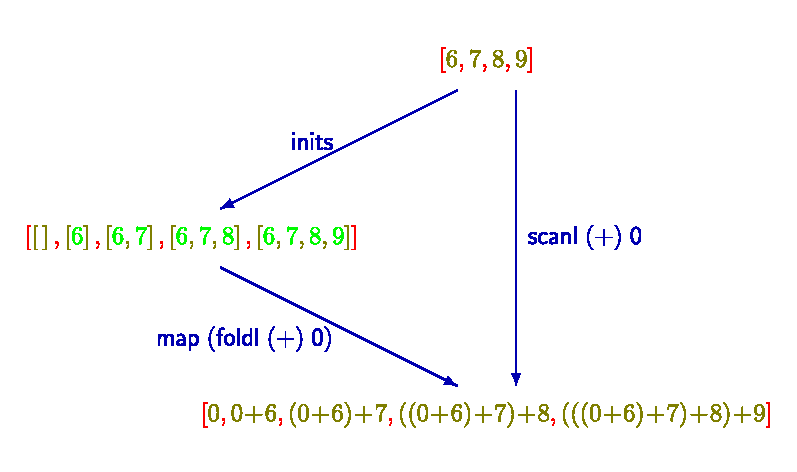
\includegraphics[width=0.9\textwidth]{scan_lemma_example.pdf}
\end{figure}

\subsection{\textit{The maximum segment sum}}

\section{Razonamiento ecuacional}

\section{Definiciones de funciones}

\section{\textit{Strict property}}



% Parece ya estar listo
\section{Analizando el tiempo}
\subsection{Notación asintótica}
\subsection{Estimando tiempo}
\subsection{Tiempo amortizado}
\subsection{Algunos ejemplos} % TODO: aquí hacer énfasis en la prog funcional

% Esta sección ya está lista
\section{Cadenas}
\subsection{Notación y terminología}
Decimos que el patrón $P$ \textbf{ocurre con un desplazamiento} $s$ en el texto $T$ si
$0 \leq s \leq n - m$ y $T[s+1 \ldots s+m] = P[1 \ldots m]$. Si $P$ ocurre con un desplazamiento
$s$ en $T$, entonces se dice que $s$ es \textbf{un desplazamiento válido}, si no, se dice que $s$
es \textbf{un desplazamiento inválido}.
El \textbf{problema de búsqueda de subcadenas} es el problema de encontrar todos los
desplazamientos válidos en los que dado el patrón $P$ ocurre en el ttexto $T$.
% aquí poner la imagen del la figura 32.1 y explicarlo

\subsection{String matching} % TODO: ver si dejarlo o cambiarlo al español
En diversas situaciones se necesita encontrar todas las ocurrencias de un patrón en un texto;
éstas pueden ir desde editores de texto hasta buscar patrones particulares en secuencias de ADN.
Es aquí cuando se hace uso de algoritmos eficientes para este problema.

Es aquí cuando se formaliza el problema de ``búsqueda de subcadenas'' (string-matching).
Supongamos que el texto es un arreglo $T[1 \ldots n]$ de longitud $n$ y el patrón es un arreglo
$P[1 \ldots m]$ de longitud $m \leq n$. También supongamos que los elementos de $P$ y $T$ son
caracteres tomados de un alfabeto finito $\Sigma$. El arreglo de caracteres $P$ y $T$ también son
llamados \textbf{cadenas} de caracteres.



Denotemos a $\Sigma^*$ como el conjunto de todas las cadenas de longitud finita formadas usando
caracteres del alfabeto $\Sigma$. La cadena de longitud cero es \textbf{la cadena vacía}, denotada
como $\varepsilon$, que también pertenece a $\Sigma^*$. La longitud de una cadena $x$ se denota
como $\vert x \vert$. La \textbf{concatenación} de dos cadenas $x$ y $y$, se denota como $xy$ y
tiene como longitud $\vert x \vert + \vert y \vert$ y consiste de los caracteres de $x$ seguidos
por los caracteres de $y$.

Decimos que una cadena $w$ es \textbf{prefijo} de una cadena $x$, denotada como $w \sqsubset x$, si
$x = wy$ para alguna cadena $y \in \Sigma^*$. Notemos que si $w \sqsubset x$, entonces
$\vert w \vert \leq \vert x \vert$. De manera análoga, decimos que una cadena $w$ es \textbf{sufijo}
de una cadena $x$, denotado como $w \sqsupset x$, si $x = yw$ para alguna $y \in \Sigma^*$. Y así
como con el prefijo, si $w \sqsubset x$, entonces $\vert w \vert \leq \vert x \vert$.
Por ejemplo, tomemos \texttt{ab $\sqsubset$ abcca} y \texttt{cca $\sqsupset$ abcca}. La cadena
vacía $\varepsilon$ es tanto un sufijo coomo un prefijo para cualquier cadena.

\subsection{Algunos algoritmos comunes de búsqueda de subcadenas}

\subsection{Problemas} % TODO: ver si dejo esto aquí lo muevo y cambiar el título

\begin{tcolorbox}
  \hypertarget{repetition_factor}{32.1 a.}
  \textbf{String matching based on repetition factors}
  Let $y^i$ denote the concatenation of string y with itself $i$ times. For example,
  \texttt{ab}$^3 =$ \texttt{ababab}. We say that a string $x \in \Sigma^*$
  \textbf{has repetition factor} $r$ if $x = y^r$ for some string $y \in \Sigma^*$ and some $r > 0$.
  Let $\rho(x)$ denote the largest $r$ such that $x$ has repetition factor $r$.
  Give an efficient algorithm that takes as input a pattern $P[1 \ldots m]$ and computes the value
  $\rho(x)$ for $i = 1,2,\ldots,m$. What is the running time of your algorithm?
  \end{tcolorbox}
  
  Lo primero que se debe de hacer es calcular la función de error $\pi$ teniendo una complejidad en
  tiempo de $\Theta(m)$ y lineal en espacio. Teniendo calculada $\pi$, consideremos $m$ la longitud
  del patrón y supongamos que $r = m - \pi[m]$ es la longitud de la $i$-esima raíz del patrón y que
  $\pi[i] = i - r$ donde $r \mid m$ es la $\frac{i}{k}$-ésima concatenación de la raíz del patrón
  hasta la $i$-ésima posición. Conlcuyendo así que $\rho(P) = \frac{m}{r}$.
  
  En otro caso, supongamos que no se cumple lo anterior, i.e., que $r \nmid m$ entonces su factor de
  repetición forzosamente debe ser 1. Por contradicción, supongamos que tiene un factor de repetición
  mayor estrico que 1 lo que significaría que tendría que habría una cadena $y^r$ y que
  $\pi[i] \geq \vert x^{r-1} \vert$, pero significaría que podríamos escribir a $x$ concatenada $r$
  veces. $\Rightarrow\!\Leftarrow$.
  
  
  \begin{tcolorbox}
  \hypertarget{cyclic_rotation}{32.4-7}   
  Give a linear-time algorithm to determine whether a text $T$ is a cyclic rotation of another string
  $T'$ . For example, \texttt{arc} and \texttt{car} are cyclic rotations of each other.
  \end{tcolorbox}
  
  Descartemos el caso en que la longitud de $T$ y $T'$ sean diferentes porque no podría ser una
  rotación cíclica. Entonces $\vert T \vert = \vert T' \vert$, sea $S = TT$ el texto donde $T$ está
  concatenado dos veces, y $P = T'$ el patrón. Usando el algoritmo de Knuth-Morris-Pratt se buscará
  el patrón $P$ en $S$ en tiempo lineal.
  
  Supongamos que $P$ aparece en $T$ desplazado $s$ posiciones a la izquierda donde
  $0 \leq s < \vert P \vert$. Si $s = 0$ entonces $T = T'$, el caso interesante es cuando $s > 0$,
  teniendo así que $T[0 \ldots s]$ es sufijo de $T'$ y $T[s+1 \ldots m]$ es prefijo de $T$. 
  
  \noindent\rule{\textwidth}{1pt}
  
  Los problemas anteriores se obtuvieron del libro \textit{Introduction to Algorithms, Third
  Edition}\cite{cormen_2009}, pero en el \autoref{chap:jueces} se verá que éstos mismos problemas
  pueden llegar a aparecer en problemas de programación competitiva, por lo que no basta con
  ``memorizar los algoritmos'' como muchos podrían llegar a pensar.
  

% Misc que tal vez podríia utilizar
% TODO: aquí agarrar cosas del polymorphic en la parte que dice: on compositioin https://wiki.haskell.org/Tutorials/Programming_Haskell/String_IO
% TODO: https://www.khanacademy.org/computing/computer-science/algorithms/asymptotic-notation/a/asymptotic-notation